% Drawing 154/06-25 -- folder 154, batch 06, archive page 110 (PDF page 111).
% Transcription: en haut à gauche, un grand dessin en couleur de la bande supersingulière : deux droites horizontales (vert foncé et vert clair), une ligne médiane en tirets, quatre verticales vert clair, des droites rouges qui se croisent en sabliers et en losanges, et de grands arcs rouges en haut et en bas ; légendes « $n - 1$ », « $\nu' - 1$ », « $\nu - 1$ », « $(n-1) - (\nu - 1) - (\nu' - 1)$ », et, à droite, « $n - \nu$ », « $(\nu - 1)$ », « $\nu$ »
% Kind: supersingular strip: lenses, hourglasses and lozenges. Method 2 (schematic redraw from the facsimile). Status: ok.
% Notes: Four light green verticals; the upper horizontal dark green, the lower one light green, a dashed median between them; red arcs: a lens between the first two verticals at the top, a wave between the second and third (top and bottom), a lens between the third and fourth (top and bottom); between the second and third verticals two red crossings on the median and a vertical stroke; between the third and fourth two verticals and two lozenges; a short blue tick at the top of each vertical and a dark mark where each vertical meets the median. Legends as the transcription reads them, placed as on the page. Redrawn 2026-11-12 (issue 128): to check again. 2026-11-14, Claude Opus 5.5, overlay check (issue 147): rasterised from its own coordinates over the 400 dpi colour scan (402 ppi native) on a unit grid; not compiled (no TeX in the session). Corrected on crops at 30 px per unit: the red strokes between the verticals were drawn as plain crossings and full-height lozenges; on the page each pair of strokes leaves from one point at the top, crosses once between the two horizontals and, in the right section, closes again at one point at the bottom (two lozenges stacked on the crossing), and the right group has a third, straight stroke down its middle; the strokes of the middle section stop on the light green line; the single strokes at x = 61 and 74 are broken where they cross the dark green line. The dark green line is solid on the left, dashed over light green between the second and third verticals, solid to the fourth and light green beyond; it carries three black dots (at x = 13.7 and on the third and fourth verticals), now drawn. The third and fourth verticals moved onto their ink (0.7 and 1 unit off), with the ends of the red arcs; the short red tails where the lens arcs meet at the ends of the waves are added. Laid over the scan again, every element lies on its ink to within about 1 unit. Status set to ok.
% Coordinates: 1 unit = 1 mm = 1/100 of the crop width (bbox in page fractions: [0.135, 0.11, 0.52, 0.225]).
% Redrawn by Claude (claude-fable-5-2), issue #128, 2026-11-12; not checked by a human; not compiled (no TeX in the session).
% Checked by Claude (claude-opus-5-5) 2026-11-14 (issue #147): overlaid on the 400 dpi colour facsimile; not compiled (no TeX in the session). Not checked by a human. Status: ok.
% Rights: reproduces part of the work -- behind RENDER_TRANSCRIPTS, never published by itself.
\documentclass[tikz,border=3pt]{standalone}
\usepackage{amsmath,amssymb}
\usetikzlibrary{patterns,arrows.meta}
\tikzset{Lg/.style={green!60!black!70}, Dg/.style={green!45!black}, Rd/.style={red!85!black}, Bl/.style={blue!70!black}, pencil/.style={black!45}, struck/.style={black!35}, mpt/.style={circle,draw,inner sep=1.3pt}, pt/.style={circle,fill,inner sep=0.9pt}, opt/.style={circle,draw,fill=white,inner sep=1.1pt}}
\begin{document}
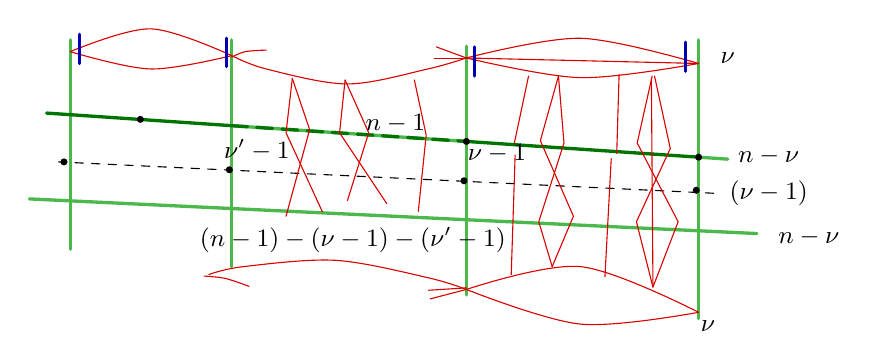
\begin{tikzpicture}[x=1mm,y=1mm,line cap=round,line join=round,font=\scriptsize]
\draw[Lg,very thick] (4.8,-5.9) -- (4.8,-32.5);
\draw[Lg,very thick] (25.3,-5.9) -- (25.3,-34.7);
\draw[Lg,very thick] (55.1,-6.7) -- (55.1,-38.3);
\draw[Lg,very thick] (84.6,-5.9) -- (84.6,-41.3);
\draw[Dg,very thick] (1.8,-15.2) -- (25.3,-16.8);
\draw[Lg,very thick] (25.3,-16.8) -- (55.1,-18.8);
\draw[Dg,very thick,dash pattern=on 5.7pt off 3.4pt] (25.3,-16.8) -- (55.1,-18.8);
\draw[Dg,very thick] (55.1,-18.8) -- (84.6,-20.8);
\draw[Lg,very thick] (84.6,-20.8) -- (88.3,-21.05);
\node[pt] at (13.7,-16) {};
\node[pt] at (55.1,-18.8) {};
\node[pt] at (84.6,-20.8) {};
\draw[Lg,very thick] (-0.4,-26.1) -- (92,-30.5);
\draw[dashed] (3.3,-21.4) -- (86.9,-25.4);
\draw[Rd] plot[smooth, tension=0.55] coordinates {(4.8,-7.4) (15,-4.5) (25.3,-7.9)};
\draw[Rd] plot[smooth, tension=0.55] coordinates {(4.8,-7.4) (15,-9.6) (25.3,-7.9)};
\draw[Rd] plot[smooth, tension=0.55] coordinates {(25.3,-7.9) (29.7,-9.6) (40,-11.5) (50.2,-9.6) (55.1,-8.2)};
\draw[Rd] plot[smooth, tension=0.55] coordinates {(55.1,-8.2) (69.6,-5.7) (84.6,-8.9)};
\draw[Rd] plot[smooth, tension=0.55] coordinates {(55.1,-8.2) (69.6,-10.7) (84.6,-8.9)};
\draw[Rd] (55.1,-8.2) -- (84.6,-8.9);
\draw[Rd] plot[smooth, tension=0.55] coordinates {(22.4,-35.7) (26.8,-34.7) (38.5,-33.9) (50.2,-36.1) (55.1,-37.6)};
\draw[Rd] plot[smooth, tension=0.55] coordinates {(55.1,-37.6) (69.6,-34.7) (84.6,-40.5)};
\draw[Rd] plot[smooth, tension=0.55] coordinates {(55.1,-37.6) (69.6,-42) (84.6,-40.5)};
\draw[Rd] plot[smooth, tension=0.55] coordinates {(25.3,-8.1) (27,-7.4) (29.7,-7.2)};
\draw[Rd] plot[smooth, tension=0.55] coordinates {(21.8,-35.9) (24.5,-36.2) (27.5,-37.2)};
\draw[Rd] (55.1,-8.2) -- (51.3,-6.8);
\draw[Rd] (55.1,-8.3) -- (51,-8.3);
\draw[Rd] (55.1,-37.4) -- (50.3,-37.7);
\draw[Rd] (55.1,-37.6) -- (50.5,-38.8);
\draw[Rd] (33,-10.8) -- (32.2,-17.7) -- (36.8,-27.7);
\draw[Rd] (33,-10.8) -- (35.2,-17.3) -- (32.2,-28.3);
\draw[Rd] (39.7,-11) -- (39,-17.7) -- (45,-26.7);
\draw[Rd] (39.7,-11) -- (42.7,-17.7) -- (40,-26.3);
\draw[Rd] (48.5,-11) -- (50,-18) -- (49,-27.7);
\draw[Rd] (63,-10.5) -- (61.2,-19);
\draw[Rd] (61.3,-20.5) -- (60.8,-35.7);
\draw[Rd] (74.5,-10.3) -- (74.2,-20.3);
\draw[Rd] (73.5,-21) -- (72.7,-36);
\draw[Rd] (66.8,-10.5) -- (64.5,-18.7) -- (68.7,-28.3) -- (66,-34.7);
\draw[Rd] (66.8,-10.5) -- (67.5,-19) -- (64.3,-29) -- (66,-34.7);
\draw[Rd] (78.7,-10.5) -- (76.8,-19) -- (82,-29) -- (78.8,-37.3);
\draw[Rd] (79,-10.5) -- (81,-19.7) -- (76.7,-29) -- (78.8,-37.3);
\draw[Rd] (78.6,-10.8) -- (78.8,-37);
\draw[Bl,very thick] (6,-5.2) -- (6,-8.9);
\draw[Bl,very thick] (24.6,-5.7) -- (24.6,-9.3);
\draw[Bl,very thick] (56.1,-6.8) -- (56.1,-10.5);
\draw[Bl,very thick] (82.9,-6.2) -- (82.9,-9.9);
\node[pt] at (4,-21.4) {};
\node[pt] at (25,-22.4) {};
\node[pt] at (54.8,-23.8) {};
\node[pt] at (84.3,-25) {};
\node[inner sep=1pt] at (88.3,-8.2) {\small $\nu$};
\node[inner sep=1pt] at (93.5,-20.7) {\small $n-\nu$};
\node[inner sep=1pt] at (93.5,-25.4) {\small $(\nu-1)$};
\node[inner sep=1pt] at (98.6,-31) {\small $n-\nu$};
\node[inner sep=1pt] at (40.7,-31.3) {\small $(n-1)-(\nu-1)-(\nu'-1)$};
\node[inner sep=1pt] at (28.5,-19.9) {\small $\nu'-1$};
\node[inner sep=1pt] at (59,-20.4) {\small $\nu-1$};
\node[inner sep=1pt] at (46.1,-16.6) {\small $n-1$};
\node[inner sep=1pt] at (85.8,-42.3) {\small $\nu$};
\end{tikzpicture}
\end{document}
